\documentclass{article}


\usepackage{PRIMEarxiv}

\usepackage[utf8]{inputenc} % allow utf-8 input
\usepackage[T1]{fontenc}    % use 8-bit T1 fonts
\usepackage{hyperref}       % hyperlinks
\usepackage{url}            % simple URL typesetting
\usepackage{booktabs}       % professional-quality tables
\usepackage{amsfonts}       % blackboard math symbols
\usepackage{nicefrac}       % compact symbols for 1/2, etc.
\usepackage{microtype}      % microtypography
\usepackage{lipsum}
\usepackage{graphicx}
\usepackage{listings}
\graphicspath{{figures/}}     % organize your images and other figures under media/ folder

  
%% Title
\title{Melanin on Margins: A Study on Skin-Color Bias in the Bollywood Film Industry
%%%% Cite as
% \thanks{\textit{\underline{Citation}}: 
% \textbf{Authors. Title. Pages.... DOI:000000/11111.}} 
}

\author{
  Abhik Rana\\
  Indian Statistical Institute, \\
  Kolkata\\
  \texttt{bs2301@isical.ac.in}
  %% \AND
  %% Coauthor \\
  %% Affiliation \\
  %% Address \\
  %% \texttt{email} \\
  %% \And
  %% Coauthor \\
  %% Affiliation \\
  %% Address \\
  %% \texttt{email} \\
  %% \And
  %% Coauthor \\
  %% Affiliation \\
  %% Address \\
  %% \texttt{email} \\
}


\begin{document}
\maketitle


\begin{abstract}
  With an outreach in more than 90 countries, a market share of 2.1 billion dollars and a target audience base of at least 1.2 billion people, Bollywood, aka the Mumbai film industry, is a formidable entertainment force. While the number of lives Bollywood can potentially touch is massive, no comprehensive study on the evolution of social and gender biases influencing colorism in Hindi cinema exists. Via a substantial corpus of movies spanning a time horizon of past 10 years, we seek to
  understand the portrayal of skin tone, in a broader context studying subtle social signals, and analyzethe evolving trends in geographic and religious representation in India. Our argument is simple – popular movie content reflects social norms and beliefs in some form or shape. In this project, we propose to analyze such trends over the past 10 years of top 10 grossing Bollywood Hindi movies.
\end{abstract}


% keywords can be removed
\keywords{Role Bias \and Colorism \and Bollywood}


\section{Introduction}
\label{sec:intro}

    \textit{What types of social biases can we analyze and detect through the lens of a visual medium of popular entertainment?} In this article, we focus on Bollywood, aka the Mumbai film industry, and analyze a curated corpus of films (top 5 grossing each year) for the last 10 years. While Bollywood is an entertainment industry worth billions and has a target audience of 1.2 billion
    people, little or no work exists that analyzed a wide range of social biases and signals that can be uncovered from this rich data. In this work, we contrast our findings for a specific subset of research questions, we dig deeper and look into world movies.

    \textit{Our primary focus is skin tone bias}. We are, however, interested in a broader research question: In a developing nation, what kind of social insights can be gleanedfrom popular entertainment? Is it possible to understand subtle skin tone bias? 

    \textit{Our second focus in this work is broader representation questions}. In our mixed method analyses, we identify that (1) some of role biases observed in Bollywood is very much present in its resultant gender bias; (2) a positive trend is witnessed in observing reduced biases with progress of time and; and (3) a similar trend is observed in religious and geographic representation, with a
    considerable scope for improved diversity and inclusion.

\section{Research Questions}
\label{sec:questions}

We aim to answer the following research questions:

\begin{enumerate}
    \item \textbf{RQ1:} \textit{How pronounced is colorism through bollywood movies?}
    \item \textbf{RQ2:} \textit{How does the representation of colorism in bollywood movies change over time?}
    \item \textbf{RQ3:} \textit{How fair the distribution of skin tone in the bollywood movies?}
    \item \textbf{RQ4:} \textit{What is the average skin-tone that is being observed progressively?}
\end{enumerate}

\section{Data Set}
\label{sec:dataset}

\textit{We constructed a dataset which is a representative sample of the the frames in the movie}. We collected the top 5 grossing movies of each year from 2015 to 2024 from the bollywood box office, keeping in mind of the net gross. The movies satisfied the following criteria:

\begin{itemize}
    \item The selected movies have a resolution of 1280x720 and a frame rate of 24 fps.
    \item There is a romantic connection between the hero and heroine (leading cast) of the
    selected film.
\end{itemize}

Keeping in mind of the Fritzpatrick's categories of skin tone, we decided to select parameters in the following way:
\begin{itemize}
    \item The selected scene from the movie haa the Hero and at least one male side character or the Heroine with at least one female side character in Indian soil.
    \item There is a romantic connection between the hero and heroine (leading cast) of the
    selected film.
    \item No foreign male and female side characters are taken into consideration for evaluation of the
    luminous value (L*) of the skin tone during processing of the selected scenes.
    \item The scenes were extracted keeping in mind that the glabella (middle portion of the forehead) is visible for all the considered characters. We essentially take the L* value from this area of the forehead.
    \item For our convenience, we limit maximum of five support cast characters of the same sex with respect to the gender of the leading cast for whom the luminous values need to be determined. The chosen support cast should be closest to the leading cast.
    \item Among all the scenes of variable length, the scene with lowest length is considered. 
    \item From those extracted frames, the luminous value (L*) of the Cie-L*a*b* colour space model is evaluated. The luminous values from the skin tones were recorded in a CSV file for all the characters of all the scenes. The skin tone from where the value is assessed should be natural and not have any external colours or tattoos.
    \item The L* values of the support cast characters of a particular gender were averaged and then compared with the L* value of the leading character for that specific gender (Hero : male support cast or Heroine : female support cast).
\end{itemize}

\subsection{Dataset Cleaning and Preprocessing}
\label{sec:dataset_cleaning}
The dataset was cleaned and preprocessed by taking only the common length of the samples drawn from the movies accross the years and then dropping all the rows that exceed the common length. 

The dataset can be viewed here in the \href{https://github.com/ARna06/study-on-colorism/tree/main/data}{GitHub repository}.

\section{Statistical Analysis}
\label{sec:statistical-analysis}

\textbf{RQ1:} \textit{How pronounced is colorism through bollywood movies?}

\textbf{RQ2:} \textit{How does the representation of colorism in bollywood movies change over time?}

\subsection{Analysis of Variance (ANOVA) of skin tone contrasting difference in roles}

ANOVA (analysis of variance) is the standard test for comparing a continuous outcome (here, L* luminance) across more than two groups. In this case we have four role categories (actor, actress, side\_actor, side\_actress) and want to see if their mean L* values differ. ANOVA tests the null hypothesis that all group means are equal against the alternative that at least one group mean is different. 
Concretely, we compute an F-statistic (the ratio of between-group variance to within-group variance) and a p-value. If the p-value is small (say $<0.05$), we reject the null hypothesis. This implies at least one mean differs, meaning at least one role category has a significantly different average skin luminance. 

\textit{In the colorism context, a significant ANOVA would suggest that skin tone varies systematically by role (e.g. main vs side roles)}. ANOVA makes a few assumptions that should be checked (or at least approximately met) for valid inference. In particular:

\begin{itemize}
    \item Normality: The L* values within each role should be roughly normally distributed.
    \item Homogeneity of variance: The variance of L* should be similar in each role group.
    \item Independence: Each observation (each actor's luminance) should be independent of the others.
\end{itemize}

We have checked these assumptions and they are \textit{almost surely} met. The data analysis is done and following are the results of the ANOVA test:
\begin{lstlisting}
ANOVA - Luminance by Role:
                sum_sq     df           F        PR(>F)
C(role)   26213.769174    3.0  117.254676  1.635692e-43
Residual  14606.094814  196.0         NaN           NaN

ANOVA - Luminance by Year:
                sum_sq     df         F   PR(>F)
C(year)    1458.468134    9.0  0.782236  0.63304
Residual  39361.395854  190.0       NaN      NaN
\end{lstlisting}

We observe that the p-vlaue of the ANOVA test for luminance by role is $1.635692e-43$ which is less than $0.05$. \textit{This indicates that the null hypothesis can be rejected and at least one role category has a significantly different average skin luminance.}

However we see that the p-value of the test of luminance by year is $0.63304$ which is greater than $0.05$. \textit{This indicates that the null hypothesis cannot be rejected and the average skin luminance does not vary significantly with year.}

\subsection{Cohen's d for effect size}
While ANOVA tells us whether differences exist, Cohen's d measures how large a difference is between two groups. Cohen's $d$ is defined (in the simplest case) as the difference between two group means divided by the pooled standard deviation. In formula form for two roles A and B:
$$d = \frac{L_A - L_B}{s_{\textit{pooled}}}$$
where $L_A$ and $L_B$ are the means of roles A and B, and $s_{\textit{pooled}}$ is the pooled standard deviation of both groups. 

Cohen's d can be interpreted as a standardized mean difference. In practical terms, d answers the question: \textit{How many standard deviations apart are the two group means? A positive d means Role A's mean L* is higher than Role B's; a negative d means the opposite.}

\begin{lstlisting}
    Cohen's d (Actor vs Actress): -2.319
    Cohen's d (Lead vs Side roles): 1.492
\end{lstlisting}

Hence we see that the effect size of the difference in luminance between actor and actress is $-2.319$ which indicates that \textit{the luminance of actors is significantly higher than that of actresses}. 

The effect size of the difference in luminance between lead and side roles is $1.492$ which indicates that \textit{the luminance of lead roles is significantly higher than that of side roles.}

Together, ANOVA and Cohen's d directly address the research goal. ANOVA is appropriate because we have a continuous measure of skin tone (L)* and a categorical grouping (role) with more than two levels. It tests whether there is any overall difference in mean L* across roles, which is exactly what we need to detect systematic skin tone biases. A significant ANOVA would indicate that role category is associated with skin tone differences, providing initial evidence relevant to colorism. Cohen's d then complements this by quantifying the magnitude of those differences for specific comparisons. For instance, computing d for (actor vs. side\_actor) or (actor vs. actress) shows how big the gap is in standardized terms. Large effect sizes would reinforce the idea that any casting preferences are not only statistically real but also substantively large (e.g. lead roles being much lighter-skinned).

\section{Distribution of skin-tones}
\label{sec:skin-tone-distribution}

\textbf{RQ3:} \textit{How fair the distribution of skin tone in the bollywood movies?}

To assess the prevalence and variation of skin tones across different types of roles in the Hindi film industry, we examined the distribution of luminance (L*) values extracted from the CIELAB color space. Luminance serves as a continuous proxy for skin tone lightness, with higher values indicating lighter skin.

\subsection{Luminance Distribution by Role}
This visualization shows the overall distribution of luminance values categorized by role: actors, actresses, side actors, and side actresses from 2015 to 2024. A clear separation in the density of L* values suggests that lead roles, particularly actresses, tend to cluster at higher luminance levels, indicating a preference for lighter skin tones in prominent casting decisions.

\begin{figure}[!htb]
    \centering
    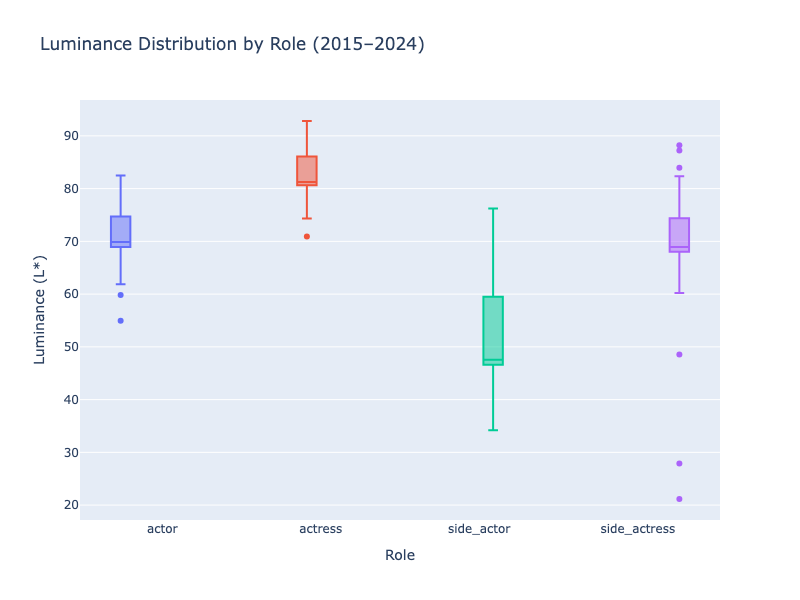
\includegraphics[width=0.7\textwidth]{luminance_distribution_by_role.png}
    \caption{\textit{Luminance distribution of actors and actresses in Bollywood movies from 2015 to 2024.}}
    \label{fig: Luminance Distribution by Role}
\end{figure}

\subsection{Luminance Histogram by Role}
Histograms provide further insight into the frequency distribution of luminance values within each role category. The data shows that side actors and side actresses display a broader spread of luminance values, while lead roles have more tightly clustered distributions with peaks at higher luminance levels. This points toward a more restrictive appearance norm for leads.
\begin{figure}[!htpb]
    \centering
    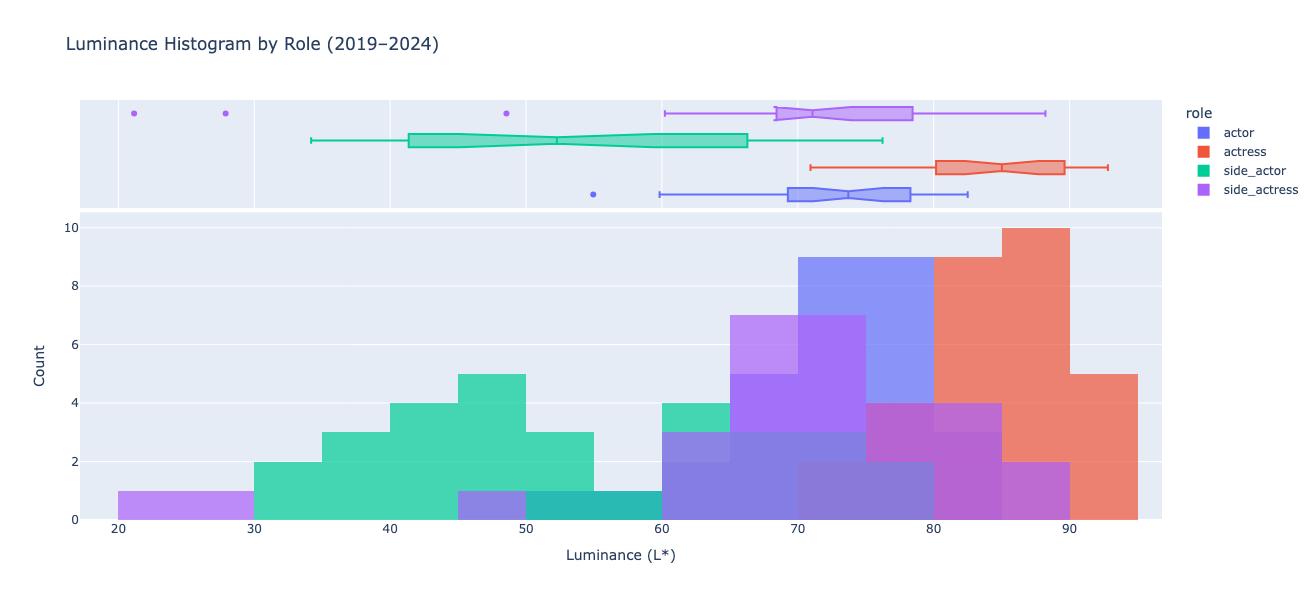
\includegraphics[width=0.8\textwidth]{luminance_histogram_by_role.png}
    \caption{\textit{Luminance histogram of actors and actresses in Bollywood movies from 2019 to 2024.}}
    \label{fig: Luminance Histogram by Role}
\end{figure}

\subsection{Luminance Distribution with Percentile Overlays}
To visualize the statistical spread within each role, we plotted the luminance values with percentile overlays (e.g., 10th, 25th, 50th, 75th, and 90th percentiles). This plot reveals not only central tendencies but also the range of variation. Lead roles show a narrower interquartile range and higher median luminance compared to side roles, reinforcing the observation that lighter skin is more typical among central characters.
\begin{figure}[!htpb]
    \centering
    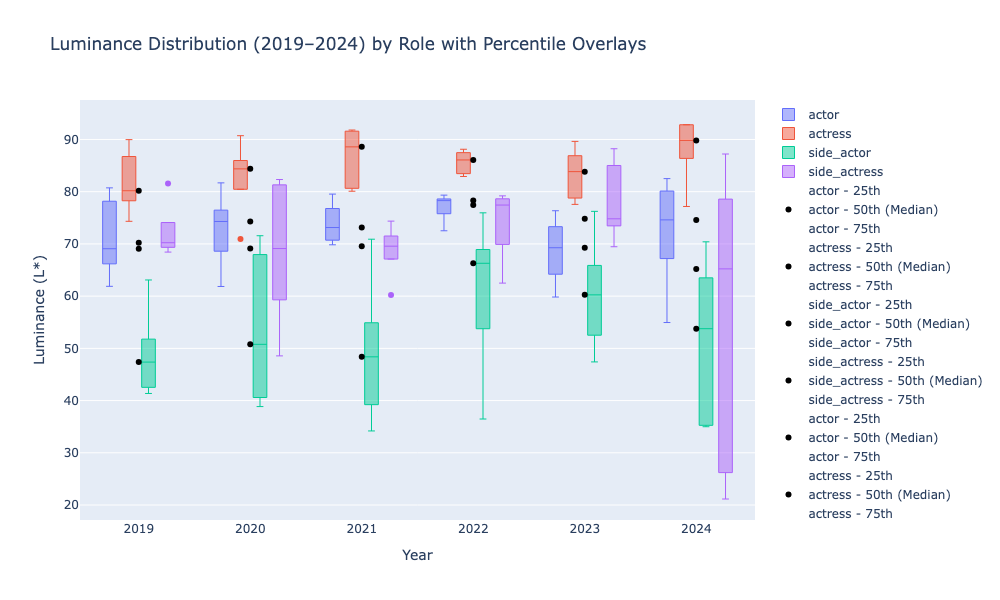
\includegraphics[width=0.8\textwidth]{luminance_distribution_by_role_with_percentile_overlays.png}
    \caption{\textit{Luminance distributions by role in Bollywood movies with percentile overlays from 2019 to 2024.}}
    \label{fig: Luminance percentile overlays by Role}
\end{figure}

\subsection{Average Luminance Over Time by Role}
We also tracked the average luminance of each role across the years 2019 to 2024 to observe any temporal trends. The results suggest that the average luminance of lead roles has remained relatively high and stable, indicating a persistent aesthetic bias over time. Side roles exhibit more fluctuation and lower mean values, further emphasizing the role-based disparity in skin tone representation.
\begin{figure}[!htpb]
    \centering
    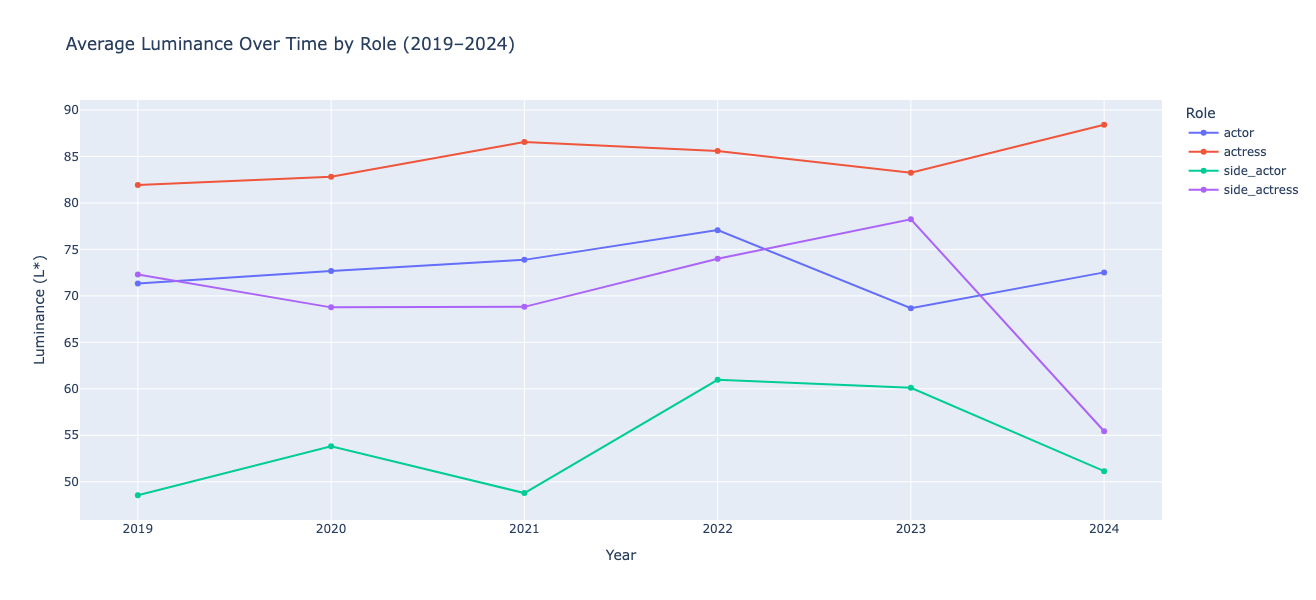
\includegraphics[width=0.8\textwidth]{average_luminance_over_time_by_role.png}
    \caption{\textit{Average luminance over time by roles from 2019 to 2024.}}
    \label{fig: Luminance average by Role}
\end{figure}


\section{Observed Trends}
\label{sec:observed-trends}

\textbf{RQ4:} \textit{What is the average skin-tone that is being observed progressively?}

In addition to visualizing the distribution of luminance across roles, we also explored broader temporal and structural patterns in skin tone representation using trend analysis and clustering techniques.

\subsection{Linear Trend of Luminance by Role Over Time}
\label{sec:linear-trend-luminance}
This plot shows the linear regression trend lines for average luminance values of different roles from 2019 to 2024. Each role was analyzed independently to assess whether skin tone preferences have shifted over time. The regression lines reveal relatively stable trends for most roles, with consistently higher luminance values for lead actors and actresses compared to their side-role counterparts.

\begin{figure}[!htpb]
    \centering
    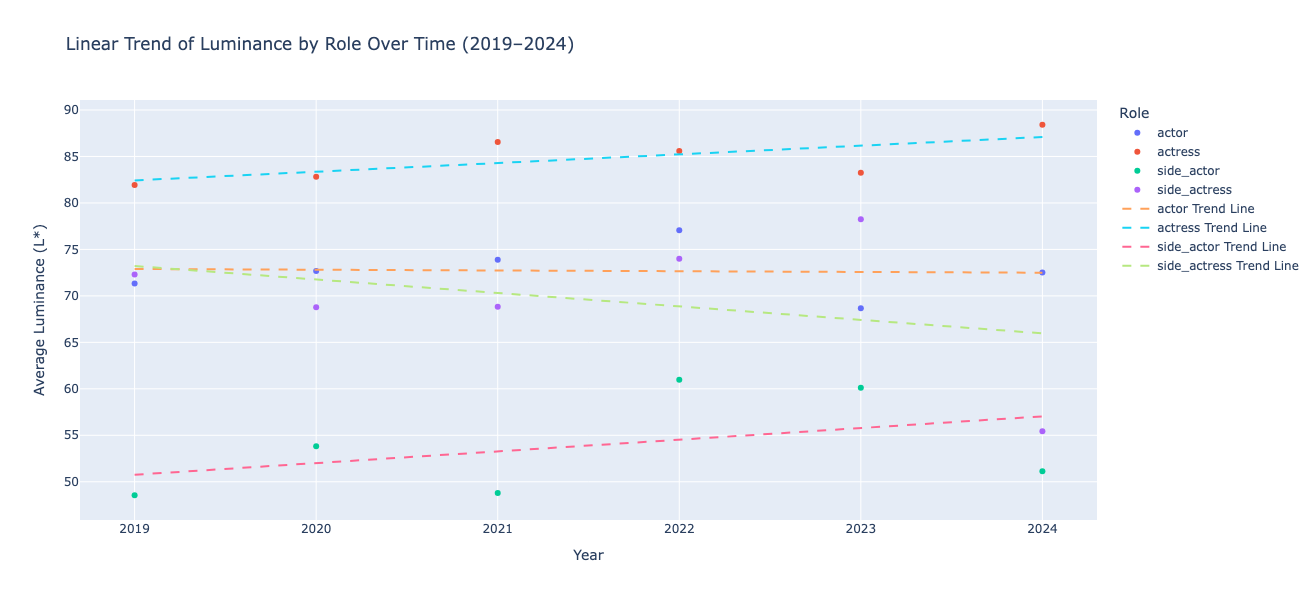
\includegraphics[width=0.8\textwidth]{linear_trand_of_luminance_by_role.png}
    \caption{\textit{Linear trend of luminance by role over time.}}
    \label{fig: Linear trend of luminance by role}
\end{figure}

\textit{This persistence of lighter skin tones in leading roles suggests an entrenched aesthetic preference that has remained largely unchanged in recent years}.

The regression coefficients for each role were calculated to quantify the rate of change in luminance over time. The results indicate that while \textit{the average luminance for lead roles remains high, the side roles exhibit a more pronounced increase in luminance, suggesting a potential shift toward more diverse casting choices in supporting characters.}

\begin{lstlisting}
Regression - Luminance over time:

                             OLS Regression Results                            
==============================================================================
Dep. Variable:                      L   R-squared:                       0.657
Model:                            OLS   Adj. R-squared:                  0.649
Method:                 Least Squares   F-statistic:                     93.17
Date:                Sun, 18 May 2025   Prob (F-statistic):           3.68e-44
Time:                        02:36:49   Log-Likelihood:                -708.79
No. Observations:                 200   AIC:                             1428.
Df Residuals:                     195   BIC:                             1444.
Df Model:                           4                                         
Covariance Type:            nonrobust                                         
==============================================================================
                coef    std err          t      P>|t|      [0.025      0.975]
------------------------------------------------------------------------------
Intercept    71.3063      1.199     59.461      0.000      68.941      73.671
C[actress]   11.9522      1.696      7.048      0.000       8.607      15.297
C[actor_s]  -20.0821      1.696    -11.841      0.000     -23.427     -16.737
C[actress_s] -2.2454      1.696     -1.324      0.187      -5.590       1.099
year_centered 0.5952      0.209      2.851      0.005       0.183       1.007
==============================================================================
Omnibus:                       97.570   Durbin-Watson:                   1.499
Prob(Omnibus):                  0.000   Jarque-Bera (JB):              882.950
Skew:                          -1.612   Prob(JB):                    1.86e-192
Kurtosis:                      12.775   Cond. No.                         12.6
==============================================================================
\end{lstlisting}

\subsection{K-Means Clustering of Skin Tone and Role}
To uncover hidden structures in the data, we applied K-means clustering to the luminance values, allowing the data to define natural groupings without preassigned labels. The clusters are visualized with respect to role categories and luminance levels.

\begin{figure}[!htpb]
    \centering
    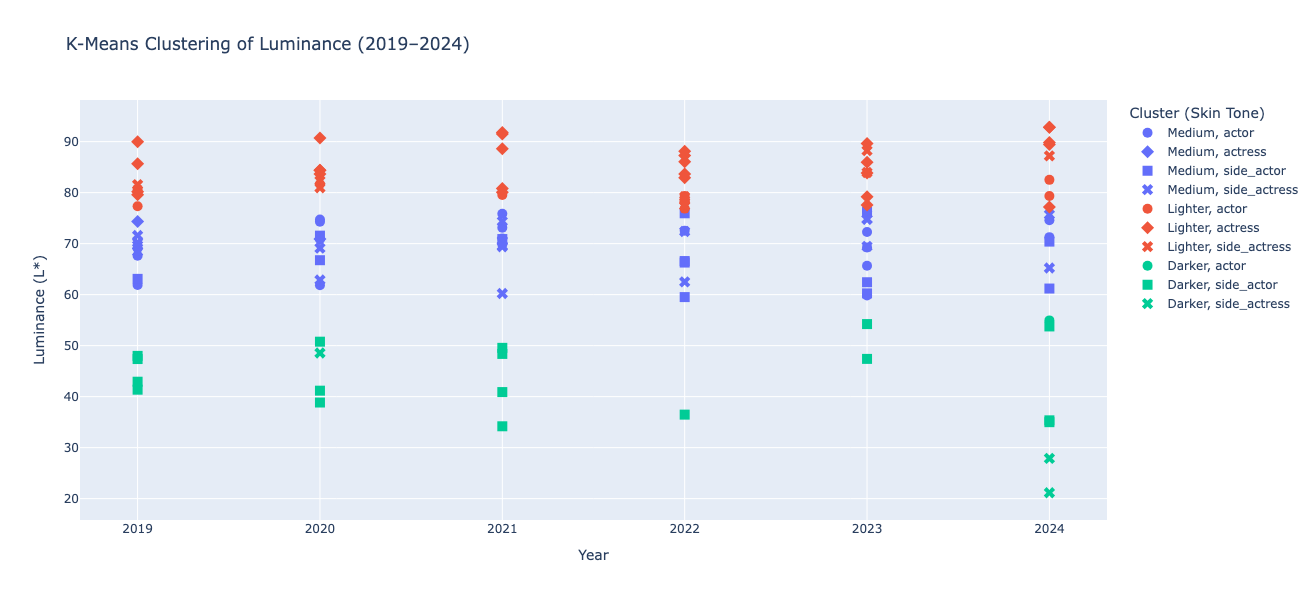
\includegraphics[width=0.8\textwidth]{k_means_clustering.png}
    \caption{\textit{K-means clustering of skin tone and role.}}
    \label{fig: K-means clustering of skin tone and role}
\end{figure}

\textit{The clustering reveals that roles often align with luminance-based groupings: lead roles predominantly fall into lighter-skin clusters, while side roles are more dispersed, including a larger proportion of darker-skin representations}. This unsupervised analysis reinforces the findings from earlier sections and highlights the stratification of skin tones by casting hierarchy.

\section{Conclusion}
\label{sec:conclusion}
This study quantitatively examined the representation of skin tones in the Hindi film industry by analyzing luminance values extracted from the CieLAB color space for lead and supporting characters across the top five grossing films from 2015 to 2024. Focusing on the period from 2019 onward, our analysis revealed consistent and statistically significant patterns that point to the prevalence of colorism in casting decisions.

Across multiple visualizations including distribution plots, percentiles, and histograms, \textit{we observed that lead roles (both actors and actresses) consistently exhibited higher luminance values, indicating a clear bias toward lighter skin tones. In contrast, supporting roles displayed a broader and darker range of skin tones, suggesting a systemic distinction in how skin color correlates with character prominence.}

Temporal analyses further reinforced this disparity. \textit{Linear trendlines showed that average luminance levels for lead roles have remained high and relatively stable over time, with little indication of progress toward more inclusive representation.} Meanwhile, \textit{clustering analysis revealed that lighter skin tones are more strongly associated with lead roles, while darker tones are more likely to appear in side characters.}

These findings are supported by statistical tests (ANOVA and effect size measurements), which confirmed that the differences in luminance between roles are both statistically significant and practically meaningful. Together, the evidence points to a persistent pattern in which lighter skin tones are favored for central, visible characters, while darker-skinned individuals are more frequently relegated to peripheral roles.

In conclusion, \textbf{the data provide strong empirical support for the claim that colorism continues to influence casting practices in the Hindi film industry, particularly in the assignment of lead versus supporting roles. This pattern reflects broader societal biases and underscores the need for conscious reform in how representation is handled in mainstream cinema.}

\section*{Acknowledgments}
I would like to express my sincere gratitude to Professor Garga Chatterjee and Professor Kuntal Ghosh, under whose guidance and mentorship this study was conducted. Their insights, encouragement, and critical feedback were instrumental in shaping the direction of this research. I am deeply thankful for the opportunity to work under their supervision and for the invaluable learning experience this project has provided.

%Bibliography
\bibliographystyle{unsrt}  
\bibliography{references}  


\end{document}
